% !TeX root=../main.tex
\chapter{تعاریف و دانش پیش‌زمینه}
%\thispagestyle{empty} 
\section{مقدمه}
در این فصل مفاهیم مورد نیاز و استفاده در این پروژه مورد بررسی قرار می‌گیرند.
این فصل شامل ۵ بخش است.
ابتدا مفاهیم کلی شبکه‌های مبتنی بر نرم‌افزار بررسی می‌شوند.
سپس زبان‌های نت‌کت
و نت‌کت پویا
که زبان‌های مورد استفاده در این تحقیق هستند شرح داده می‌شوند.
در ادامه تعاریف اولیه ساختمان‌رویداد
\lf{Event Structure}
که به عنوان مدل معنایی در این تحقیق استفاده می‌شود شرح داده می‌شود.
در بخش آخر مدل علّی
\lf{Causal Model}
که در این تحقیق برای پیدا کردن علت واقعی خطا مورد استفاده قرار می‌گیرد توصیف شده است.


\section{شبکه‌های مبتنی بر نرم‌افزار}
شبکه‌های کامپیوتری یکی از زیر‌ساخت‌های حیاتی سیستم‌های کامپیوتری هستند.
با وجود اینکه نیازمندی‌های این شبکه‌ها بسیار بیشتر و پیشرفته‌تر نسبت به گذشته شده است تکنیک‌ها و متد‌های مدیریت و ساخت آن‌ها همچنان مانند گذشته است. 
این مساله مدیریت آن‌ها را در استفاده‌های امروزی پیچیده و مستعد خطا می‌کند. 
حتی شرکت‌های بزرگی مانند
Github, Amazon
یا
GoDaddy
مرتبا مشکلاتی در شبکه‌های خود پیدا می‌کنند
\cite{foerster2018survey}
.
شبکه‌های مبتنی بر نرم‌افزار
یک پارادایم جدید برای طراحی و پیاده‌سازی شبکه‌های کامپیوتری هستند که علاوه بر اینکه مدیریت و درستی‌سنجی آن‌ها را با روش‌های اصولی‌تر امکان‌پذیر می‌کنند، انعطاف بالایی هم دارند.
به صورت خلاصه در یک شبکه‌ی مبتنی بر نرم‌افزار رفتار‌های کنترلی 
(تغییر و به‌روز رسانی قوانین ارسال
\lf{Forwarding Rule}
)
از عناصر شبکه مانند سوییچ‌ها یا روترها جدا می‌شوند و توسط یک کنترل‌کننده‌ی مرکزی انجام می‌شوند.
به عنوان مثال در زبان 
OpenFlow \cite{mckeown2008openflow}
رفتار سوییچ‌های شبکه تنها توسط تعدادی قانون به شکل 
تطبیق
\lf{Match}
و اجرا
\lf{Action}
توصیف می‌شود.
قوانینی به این شکل ابتدا بررسی می‌کنند که بسته با قانون تطابق داشته باشد و اگر تطابق وجود داشت عملیات توصیف شده در قانون اجرا می‌شود.
با ساده شدن عناصر شبکه،‌ تمامی به‌روز رسانی‌ها و تغییر‌های لازم در شبکه توسط یک کنترل کننده مرکزی انجام می‌شود.
متمرکز شدن رفتار کنترلی سیستم باعث می‌شود تا استدلال و درستی سنجی در مورد رفتار شبکه آسان تر شود.

\section{نت‌کت }
نت‌کت
،یک زبان برای توصیف شبکه‌های مبتنی بر نرم‌افزار است
\cite{netkat}.
این زبان با وجود دستور زبان
\lf{Syntax}
ساده‌ای که دارد، بر اساس
KAT
\cite{kat}
بنا شده و به همین دلیل یک سیستم معادلاتی صحیح و کامل
\lf{Sound and Complete}
دارد.
این سیستم معادلاتی کمک می‌کند تا با استفاده از روش‌های جبری و اثبات تساوی برنامه‌های توصیف شده در این زبان بتوان در مورد آن‌ها استدلال کرد.

\subsection{دستور زبان نت‌کت}
در نت‌کت هر بسته
به عنوان یک نگاشت از یک مجموعه از فیلد‌های
$f_1,f_2,...,f_n$
به اعداد طبیعی با تعداد ارقام ثابت در نظر گرفته می‌شود.
آی‌پی‌
\lf{IP}
های مبدا و مقصد، نوع بسته، پورت‌
\lf{Port}
های مبدا و مقصد مثال‌هایی از این فیلد‌ها هستند.
دستور زبان نت‌کت به صورت زیر تعریف می‌شود:
\begin{align*}
    a,b ::= & 1 | 0 | f = n | a + b | a \cdot b | \neg a  \\
    p,q ::= & a | f \la n | p + q | p \cdot q | p^* | dup
\end{align*}
در این گرامر عبارت‌های
$a,b$
عملا معادل با تست‌های زبان کت
\lf{KAT}
هستند.
عبارت‌های
$p,q$
عبارت‌های نت‌کت را تعریف می‌کنند که نسبت به دستور زبان کت
جمله‌هایی به شکل
$dup$
و
$f \la n$
به آن اضافه شده است.
\subsection{مدل معنایی نت‌کت}
برای اینکه امکان استدلال در مورد مسیر‌های طی شده توسط یک بسته‌ در شبکه وجود داشته باشد،از مفهومی به نام تاریخچه‌ی بسته
\lf{Packet History}
استفاده می‌شود.
هر تاریخچه‌ی بسته‌، یک دنباله از بسته‌ها است که بسته نخست دنباله، به عنوان بسته‌ی فعلی در نظر گرفته می‌شود.
به صورت شهودی
عبارت های ۱ و ۰ به ترتیب به معنای ارسال
\lf{Forward}
و رها کردن
\lf{Drop}
بدون شرط بسته هستند.
عبارت
$f=n$
در صورتی بسته را عبور می‌دهد که مقدار فیلد
f
آن برابر با
n
باشد.
عبارت
$f \la n$
مقدار n
را به فیلد f
بسته اختصاص
می‌دهد.
عبارت‌های
$dup$
باعث می‌شوند تا یک کپی از بسته‌ی فعلی ایجاد شود و به تاریخچه‌ی بسته‌ها اضافه شود.
این عبارات در رفتار شبکه تاثیری ندارند اما امکان استدلال در مورد تمامی تغییرات ایجاد شده در حین جا‌به‌جایی بسته در شبکه را فراهم می‌سازند.
به صورت دقیق، معنای هر عبارت
\lf{Expression}
نت‌کت با استفاده از معادلات زیر تعریف می‌شود:
\begin{align}
    \sem{p}             & H \in \mathcal{P}({H}) \label{eq:netkat:sem}                  \\
    \sem{1} h           & \teq \s{h}     \label{eq:netkat:identity}                     \\
    \sem{0} h           & \teq \s{}          \label{eq:netkat:drop}                     \\
    \sem{f=n}(pk::h)    & \teq \begin{cases}
                                   \s{pk::h} & \text{ if } pk.f = n \\
                                   \s{}      & \text{ otherwise }
                               \end{cases}    \label{eq:netkat:filter}                  \\
    \sem{\neg a}        & \teq \s{h} \setminus (\sem{a}h) \label{eq:netkat:nfilter}     \\
    \s{f \la n} (pk::h) & \teq \s{pk[f:=n]::h}     \label{eq:netkat:assign}             \\
    \sem{p+q}h          & \teq \sem{p}h \cup \sem{q}h   \label{eq:netkat:sum}           \\
    \sem{p\cdot q} h    & \teq (\sem{p} \bullet \sem{q}) h    \label{eq:netkat:dot}     \\
    \sem{p^*}h          & \teq \bigcup_{i \in \mathbb{N}}F^i h \label{eq:netkat:kleene} \\
    F^0 h               & \teq \s{h}                                                    \\
    F^{i+1} h           & \teq (\sem{p} \bullet F^i) h                                  \\
    (f \bullet g) x     & \teq \bigcup\s{g(y)|y \in f(x)}                               \\
    \sem{dup} (pk::h)   & \teq \s{pk::(pk::h)} \label{eq:netkat:dup}
\end{align}
در معادلات بالا فرض می‌شود که 
$H$
مجموعه‌ی تمامی تاریخچه‌های ممکن است.
معادله‌ی 
\ref{eq:netkat:sem}
بیان می‌کند که معنی هر عبارت نت‌کت روی یک تاریخچه‌ی بسته یک مجموعه از  
تاریخچه‌ی بسته‌های حاصل از اعمال این عبارت روی تاریخچه‌ی ورودی است.
معادله‌ی 
\ref{eq:netkat:identity}
بیان می‌کند که عبارت ۱ بسته را بدون شرط عبور می‌دهد.
در مقابل معادله‌ی 
\ref{eq:netkat:drop}
رها شدن بسته را با خروجی یک مجموعه‌ی خالی مدل می‌کند.
معادله‌ی 
\ref{eq:netkat:filter}
بسته‌ی نخست ورودی را بررسی می‌کند و اگر مطابق با عبارت نبود بسته رها می‌شود.
معادله‌ی
\ref{eq:netkat:assign}
مقدار 
$n$
را به فیلد
$f$
بسته‌ی نخست تاریخچه اختصاص می‌دهد.
در معادله‌ی 
\ref{eq:netkat:kleene}
حاصل اپراتور ستاره‌ی کلین
\lf{Kleene Star}
معادل با اجتماع اعمال عبارت به تعداد دلخواه روی تاریخچه‌ی ورودی در نظر گرفته شده است.
در نهایت معادله‌ی 
\ref{eq:netkat:dup}
یک کپی از بسته‌ی نخست ورودی را به ابتدای خروجی اضافه می‌کند.

نت‌کت علاوه بر اصول موضوعه‌ی
\lf{Axiom}
KAT
اصول‌ موضوعه‌ی زیر را هم شامل می‌شود تا دستگاه معادلاتی صحیح و کامل
\lf{Sound and Complete}
داشته باشد:
\begin{align}
    f \la n \cdot f' \la n' & \equiv f' \la n' \cdot f \la n,
    \text{ if } f \neq f' \label{mod-mod-comm}
    \\
    f \la n \cdot f' = n'   & \equiv f' = n' \cdot f \la n,
    \text{ if } f \neq f' \label{mod-filter-comm}                            \\
    dup \cdot f = n         & \equiv f = n \cdot dup \label{dup-filter-comm} \\
    f \la n \cdot f = n     & \equiv f \la n \label{mod-filter}              \\
    f = n \cdot f \la n     & \equiv f = n \label{filter-mod}                \\
    f \la n \cdot f \la n'  & \equiv f \la n' \label{mod-mod}                \\
    f = n \cdot f = n'      & \equiv 0, \text{ if } n \neq n' \label{contra} \\
    \Sigma_{i} f = i        & \equiv 1 \label{match-all}
\end{align}
اصل‌های
\ref{mod-mod-comm},\ref{mod-filter-comm},\ref{dup-filter-comm}
خواص جابه‌جایی
\lf{Commutative}
عملیات‌ها را بیان می‌کنند.
اصل
\ref{mod-filter}
بیان می‌کند که اختصاص مقدار
n
به یک فیلد و سپس  فیلتر کردن بر روی این فیلد با همین مقدار معادل با عملیات اختصاص
\lf{Assignment}
به تنهایی است.
مشابه همین اصل برای یک فیلتر و سپس یک اختصاص هم در اصل
\ref{filter-mod}
مشخص شده.
اصل
\ref{mod-mod}
بیان می‌کند که در دنباله‌ای از اختصاص مقادیر به یک فیلد مشخص، تنها آخرین اختصاص تاثیر دارد.
در اصل
\ref{contra}
مشخص شده است که مقدار یک فیلد نمی‌تواند دو مقدار متفاوت داشته باشد.
در نهایت اصل
\ref{match-all}
بیان می‌کند که عملیات مجموع فیلتر‌ها به ازای هر مقدار ممکن برای یک فیلد مشخص برابر عنصر همانی
\lf{Identity}
است.

\subsection{توصیف رفتار شبکه با نت‌کت}

در ادامه نحوه‌ی توصیف یک شبکه با استفاده از نت‌کت بیان می‌شود.
\begin{figure}
    \centering
    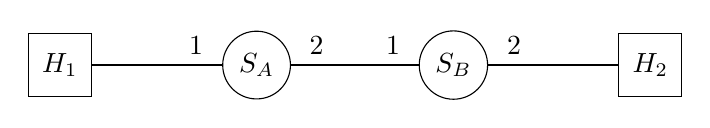
\begin{tikzpicture}[
            node distance={25mm},
            sw/.style = {draw, circle,minimum size=8mm},
            h/.style = {draw, rectangle,minimum size=8mm}
        ]
        \node[h] (h1)  {$H_1$};
        \node[sw] (sa) [right of=h1]  {$S_A$};
        \node[sw] (sb) [right of=sa] {$S_B$};
        \node[h] (h2)  [right of=sb] {$H_2$};
        \draw [thick] (h1)  -- node[above,pos=0.8]{1} (sa);
        \draw [thick] (sa) -- node[above,pos=0.2]{2}
        node[above,pos=0.8]{1}(sb);
        \draw [thick] (sb) -- node[above,pos=0.2]{2} (h2);
    \end{tikzpicture}
    \caption{مثال شبکه}
    \label{fig:netkat:ssh}
\end{figure}
در شکل
\ref{fig:netkat:ssh}
شبکه شامل دو سوییچ
\lf{Switch}
A و ‌B
و دو هاست
\lf{Host}
می‌باشد.
هر سوییچ دو پورت دارد که با شماره‌های ۱ و۲ مشخص شده‌اند.
در این شبکه هدف این است که امکان جا‌به‌جایی همه‌ی بسته‌ها به غیر از بسته‌هایی که از نوع
SSH
هستند وجود داشته باشد.
عبارت نت‌کت زیر را در نظر بگیرید:
\begin{align*}
    p \triangleq (dst = H_1 \cdot pt \la 1) +
    (dst = H_2 \cdot pt \la 2)
\end{align*}
این عبارت همه‌ی بسته‌هایی که مقصد آن‌ها هاست ۱ باشد را به پورت ۱ و همه‌ی بسته‌هایی که مقصد‌ آن‌ها هاست ۲ باشد را به پورت شماره‌ی ۲ می‌فرستد.
این سیاست
\lf{Policy}
به سادگی رفتار سوییچ‌ها را در نت‌کت تعریف می‌کند.
در ادامه می‌توان با اضافه کردن یک فیلتر به این عبارت، ویژگی دسترسی کنترل
\lf{Access Control}
را به این سیاست اضافه کرد تا همه‌ی بسته‌های از نوع
SSH
رها شوند:
\begin{align*}
    p_{AC} \triangleq \neg(typ = SSH)\cdot p
\end{align*}
اما استفاده از عبارت بالا به تنهایی برای توصیف رفتار شبکه شکل
\ref{fig:netkat:ssh}
کافی‌ نیست.
برای تکمیل این عبارت لازم است تا رفتار توپولوژی
\lf{Topology}
شبکه‌ هم به آن افزوده شود.
در نت‌کت توپولوژی شبکه به عنوان یک گراف جهت‌دار در نظر گرفته می‌شود و رفتار آن در قالب اجتماع رفتار هر یک از پیوندهای
\lf{Link}
آن توصیف می‌شود.
برای شبکه‌ی شکل
\ref{fig:netkat:ssh}
می‌توان از عبارت زیر برای توصیف توپولوژی شبکه استفاده کرد:
\begin{align*}
    t \triangleq & (sw = A \cdot pt = 2 \cdot sw \la B \cdot pt \la 1) + \\
                 & (sw = b \cdot pt = 1 \cdot sw \la A \cdot pt \la 2) + \\
                 & (sw = b \cdot pt = 2)
\end{align*}
در نت‌کت در صورتی که سیاست و توپولوژی شبکه در قالب عبارت‌هایی توصیف شده‌باشند،
رفتار کل شبکه در واقع دنباله‌ای از اعمال این عبارت‌ها به صورت یکی در میان است.
به عنوان مثال در شکل
\ref{fig:netkat:ssh}
یک بسته از هاست ۱ ابتدا توسط سوییچ
A
پردازش شده، سپس روی لینک بین دو سوییچ جا به جا می‌شود و در نهایت توسط سوییچ
B
پردازش می‌شود.
در نت‌کت می‌توان این رفتار را به صورت
$p_{AC}\cdot t \cdot p_{AC}$
توصیف کرد.
با استفاده از همین شهود، رفتار کل شبکه را می‌توان در قالب عبارت زیر توصیف کرد:
\begin{align*}
    (p_{AC}\cdot t)^*
\end{align*}
در توصیف بالا فرض شده است که بسته‌ها می‌توانند به هر طریق ممکن وارد شبکه و از آن خارج شوند، اما این رفتار همیشه مورد قبول نیست.
به عنوان مثال در شبکه شکل
\ref{fig:netkat:ssh}
اگر مکان‌های ورودی و خروجی شبکه را در قالب عبارت زیر توصیف کنیم:
\begin{align*}
    e \triangleq sw = A\cdot port = 1 \vee sw = B \cdot port = 2
\end{align*}
می‌توانیم رفتار انتها به انتهای
\lf{End to End}
شبکه را به شکل زیر توصیف کنیم:
\begin{align*}
    p_{net} \triangleq e \cdot (p_{AC}\cdot t)^* e
\end{align*}
در حالت کلی‌تر، نیازی به توصیف ورودی و خروجی‌های شبکه در قالب یک عبارت نیست.
پس اگر فرض شود که مکان‌های ورودی شبکه توسط عبارت
$in$
و مکان‌های خروجی شبکه در قالب عبارت
$out$
توصیف شده‌ باشند، رفتار یک شبکه در نت‌کت به صورت زیر تعریف می‌شود:
\begin{align*}
    in \cdot (p\cdot t)^*\cdot out
\end{align*}
که عبارت
$p$
سیاست شبکه و عبارت
$t$
توپولوژی شبکه است.

\subsection{درستی‌سنجی برنامه‌های نت‌کت}
درستی‌سنجی یک شبکه و بررسی خواص آن در نت‌کت با استفاده از بررسی تساوی عبارت یک شبکه با عبارت‌های دیگر انجام می‌شود.
به عنوان مثال در شبکه‌ی شکل
\ref{fig:netkat:ssh}
برای بررسی اینکه همه‌ی بسته‌ها با نوع
SSH
از هاست ۱ رها می‌شوند کافی است تا تساوی زیر را ثابت کنیم:
\begin{equation*}
    \begin{pmatrix}
        type = SSH \cdot sw = A \cdot pt = 1 \cdot \\
        (p_{AC}\cdot t) ^ * \cdot                  \\
        sw = B\cdot pt = 2
    \end{pmatrix}
    \equiv 0
\end{equation*}
از طرفی برای بررسی یک خاصیت در شبکه، مثلا امکان فرستاده شدن‌ همه‌ی بسته‌هایی که از نوع
SSH
نیستند از هاست ۱ به هاست ۲
می‌توان به جای بررسی تساوی دو عبارت از نامساوی
$p \leq q$
استفاده کرد.
این نامساوی که خلاصه شده‌ی تساوی
$p + q \equiv q$
است بیان می‌کند که رفتار عبارت
$p$
بخشی از رفتار عبارت
$q$
است.
بنابراین برای بررسی این مساله که شبکه‌ی شکل
\ref{fig:netkat:ssh}
بسته‌های غیر
$SSH$
از هاست ۱ را عبور می‌دهد کافی است تا درستی نامعادله‌ی زیر را بررسی کرد:
\begin{equation*}
    \begin{pmatrix}
        \neg(type = SSH) \cdot sw = A \cdot pt = 1 \cdot & \\
        sw \la B \cdot pt \la 2                          &
    \end{pmatrix}
    \leq (p_{AC}\cdot t)^ *
\end{equation*}

\section{نت‌کت پویا}
نک‌کت‌ پویا
\lf{DyNetKAT}
برای رفع برخی از کاستی‌های نت‌کت ارائه شده است
\cite{dynetkat}.
به صورت دقیق‌تر نت‌کت پویا، امکان توصیف به‌روز‌رسانی سیاست‌های شبکه و همچنین رفتار شبکه در مقابل چندین بسته را ممکن می‌سازد.

\subsection{دستور زبان نت‌کت پویا}
در نت‌کت‌ پویا، از رفتار انتها به انتها‌ی توصیف‌های شبکه در قالب عبارت‌های نت‌کت استفاده می‌شود.
به همین منظور سینتکس نت‌کت‌ پویا به صورت زیر تعریف می‌شود:
\begin{align*}
    N & :: = \mathrm{NetKAT}^{-dup}                    \\
    D & :: = \bot | N;D | x?N;D | x!N;D | D\parallel D
    D \oplus D | X                                     \\
      & X \triangleq D
\end{align*}
در سینتکس بالا
$\mathrm{NetKAT}^{-dup}$
قسمتی از زبان نت‌کت است که عبارت‌های
$dup$
از آن حذف شده است.
عبارت‌های
$dup$
در توصیف‌های نت‌کت تاثیری در رفتار یک عبارت ندارند و هدف از استفاده از آن‌ها ثبت یک اثر از هر بسته پس از پردازش توسط یکی از عناصر شبکه است و امکان استدلال بر روی رفتار شبکه را ممکن می‌سازد.
با توجه به این که در نت‌کت پویا رفتار انتها به انتهای یک عبارت نت‌کت مورد استفاده است، عبارت
$dup$
از دستور زبان کنار گذاشته شده است.
نت‌کت‌پویا یک لیست از بسته‌های ورودی را پردازش می‌کند و یک لیست از مجموعه‌ی بسته‌های خروجی تولید می‌کند.
اپراتور ترکیب متوالی
\lf{Sequential Composition}
$N;D$
باعث می‌شود که یک بسته از لیست بسته‌های ورودی توسط سیاست
$N$
پردازش شود و سپس بسته‌ی توسط عبارت
$D$
پردازش می‌شود.
در نت‌کت پویا امکان ارتباط توسط عبارت‌هایی به شکل
$x!N$
و
$x?N$
توصیف می‌شوند که به ترتیب ارسال و دریافت یک عبارت نت‌کت را روی کانال
$x$
توصیف می‌کنند.
ترکیب موازی
\lf{Parallel Composition}
دو عبارت توسط
$D \parallel D$
توصیف می‌شود.
در نهایت رفتار‌های غیرقطعی
\lf{Non-Deterministic}
توسط‌ عبارت‌هایی به شکل
$D \oplus D$
توصیف می‌شوند.

\subsection{معنای عملیاتی نت‌کت پویا}
معنای عملیاتی
\lf{Operational Seamntic}
نت‌کت پویا با استفاده از عبارت‌هایی به شکل
$(d,H,H')$
تعریف می‌شوند که
$d$
عبارت نت‌کت‌ پویا فعلی است،
$H$
لیست بسته‌هایی که در ادامه باید پردازش شوند
و
$H'$
لیست بسته‌هایی است که به صورت موفقیت‌آمیز توسط شبکه پردازش شده‌اند.
در اینجا فرض می شود که
$F = \s{f_1,...,f_n}$
یک مجموعه از فیلد‌های بسته‌ها است.
یک بسته به شکل یک تابع
$F \ra \mathbb{N}$
توصیف می‌شود.
برای یک بسته مانند
$\sigma$
تساوی
$\sigma(f_i) = v_i$
بیان می‌کند که مقدار فیلد
$f_i$
در بسته‌ی
$\sigma$
برابر با
$v_i$
است.
یک لیست خالی از بسته‌ها با
$\his{}$
نمایش داده می‌شود.
اگر
$l$
یک لیست از بسته‌ها باشد
$e::l$
لیستی است که حاصل از اضافه کردن بسته
$\sigma$
به ابتدای لیست به دست می‌آید.
برچسب هر قانون که با
$\gamma$
مشخص می‌شود به صورت یکی از شکل‌های
$(\sigma,\sigma'),x!q,x?q$
یا
$rcfg(x,q)$
تعریف می‌شود
که
$rcfg(x,q)$
به معنی انجام شدن
$x!q$
و
$x?q$
به صورت همگام
\lf{Synchronized}
است.
قوانین زیر معنای عملیاتی نت‌کت پویا را تعریف می‌کنند:
\begin{align}
     & (cpol^{\checkmark}_{\_;})
    \frac{\sigma' \in \sem{p}(\sigma::\his{})}
    {(p;q,\sigma::H,H')\xrightarrow{(\sigma,\sigma')}
    (q,H,\sigma'::H') }    \label{os:term}                                 \\
     & (cpol_X)
    \frac{(p,H_0,H_1)\xrightarrow{\gamma}(p',H_0',H_1')}
    {(X,H_0,H_1)\xrightarrow{\gamma}(p',H_0',H_1')}
    X \triangleq p         \label{os:recr}                                 \\
     & (cpol_{\_\oplus})
    \frac{(p,H_0,H_0')\xrightarrow{\gamma}(p',H_1,H_1')}
    {(p\oplus q,H_0,H_0')\xrightarrow{\gamma}(p',H_1,H_1')}
    \label{os:orr}                                                         \\
     & (cpol_{\oplus\_})
    \frac{(q,H_0,H_0')\xrightarrow{\gamma}(q',H_1,H_1')}
    {(p\oplus q,H_0,H_0')\xrightarrow{\gamma}(p',H_1,H_1')} \label{os:orl} \\
     & (cpol_{\_\parallel})
    \frac{(p,H_0,H_0')\xrightarrow{\gamma}(p',H_1,H_1')}
    {(p\parallel q,H_0,H_0')\xrightarrow{\gamma}(p' \parallel q,H_1,H_1')}
    \label{os:parr}                                                        \\
     & (cpol_{\parallel\_})
    \frac{(q,H_0,H_0')\xrightarrow{\gamma}(q',H_1,H_1')}
    {(p\parallel q,H_0,H_0')\xrightarrow{\gamma}(p \parallel q',H_1,H_1')}
    \label{os:parl}                                                        \\
     & (cpol_?)
    \frac{}
    {(x?p;q,H,H')\xrightarrow{x?p}(q,H,H')}
    \label{os:recv}                                                        \\
     & (cpol_!)
    \frac{}
    {(x!p;q,H,H')\xrightarrow{x!p}(q,H,H')}
    \label{os:send}                                                        \\
     & (cpol_{!?})
    \frac{
        (q,H,H') \xrightarrow{x!p}(q',H,H')
        (s,H,H') \xrightarrow{x?p} (s',H,H')
    }{
        (q\parallel,H,H') \xrightarrow{rcfg(x,p)} (q'\parallel s',H,H')
    }     \label{os:syncr}                                                 \\
     & (cpol_{?!})
    \frac{
        (q,H,H') \xrightarrow{x?p}(q',H,H')
        (s,H,H') \xrightarrow{x!p} (s',H,H')
    }{
        (q\parallel,H,H') \xrightarrow{rcfg(x,p)} (q'\parallel s',H,H')
    } \label{os:syncl}
\end{align}
قانون 
\ref{os:term}
انجام یک عملیات مانند
$(\sigma,\sigma')$
که به معنای
پردازش بسته‌ی ابتدایی لیست ورودی توسط عبارت 
$p$
و افزودن خروجی حاصل از آن مانند 
$\sigma'$
به لیست خروجی است را مشخص می‌کند.
قانون 
\ref{os:recr}
بیان می‌کند که رفتار متغیر 
$X$
که برابر با عبارت 
$p$
است معادل با رفتار عبارت 
$p$
است.
قوانین 
\ref{os:orr}
و
\ref{os:orl}
رفتار غیرقطعی را توصیف می‌کنند.
قوانین
\ref{os:parr}
و
\ref{os:parl}
رفتار دو عبارت موازی را توصیف می‌کنند.
قوانین
\ref{os:recv}
و
\ref{os:send}
مشخص می‌کنند که ارسال یا دریافت پیام در نت‌کت پویا پردازشی روی بسته‌ها انجام نمی‌دهد.
در نهایت همگام‌سازی
\lf{Synchronization}
ارسال و دریافت پیام توسط قوانین 
\ref{os:recv}
و
\ref{os:send}
توصیف شده است.

\subsection{توصیف برنامه‌ها در نت‌کت پویا}

\begin{figure}
    \centering
    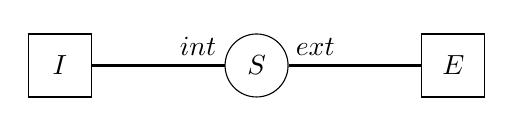
\begin{tikzpicture}[
            node distance={25mm},
            sw/.style = {draw, circle,minimum size=8mm},
            h/.style = {draw, rectangle,minimum size=8mm}
        ]
        \node[h] (i)  {$I$};
        \node[sw] (s) [right of=i]  {$S$};
        \node[h] (e)  [right of=s] {$E$};
        \draw [thick] (i)  -- node[above,pos=0.8]{$int$} (s);
        \draw [thick] (s) -- node[above,pos=0.2]{$ext$} (e);
    \end{tikzpicture}
    \caption{مثال دیوار آتش}
    \label{fig:dynetkat:firewall}
\end{figure}
در ادامه چگونگی توصیف یک دیوار آتش
\lf{Firewall}
وابسته به حالت
\lf{Stateful}
با استفاده از نت‌کت پویا بیان می‌شود.
شبکه‌ی شکل
\ref{fig:dynetkat:firewall}
را در نظر بگیرید.
در این شبکه هدف این است که امکان ارتباط از داخل شبکه به بیرون فراهم باشد ولی امکان ارسال بسته از خارج شبکه ممکن نباشد.
اما زمانی که یک بسته به خارج شبکه ارسال شد، دیوار آتش باید اجازه‌ی عبور بسته‌ها از بیرون را بدهد تا پاسخ بسته‌ها دریافت شوند.
برای توصیف این شبکه می‌توان از عبارت نت‌کت پویای زیر استفاده کرد:
\begin{align*}
    Host  \triangleq   & secConReq!1;Host \oplus secConEnd!1;Host        \\
    Switch \triangleq  & (port = int) \cdot (port \la ext);Switch \oplus \\
                       & (port = ext)\cdot 0 ; Switch \oplus             \\
                       & secConReq?1;Switch'                             \\
    Switch' \triangleq & (port =int) \cdot (port \la ext);Switch' \oplus \\
                       & (port=ext)\cdot(port\la int);Switch' \oplus     \\
                       & secConEnd?1;Switch                              \\
    Init \triangleq    & Host \parallel Switch
\end{align*}
در این توصیف عملیات 
$secConReq$
برای شروع ارتباط امن و
$secConEnd$
برای خاتمه‌ی ارتباط امن در نظر گرفته شده‌است.
بنابراین برنامه‌ی سوییچ پس از دریافت پیام برای شروع ارتباط امن تبدیل به برنامه‌ی 
$Switch'$
می‌شود که در آن اجازه‌ی ارسال بسته از پورت خارجی به پورت داخلی را دارد.
پس از دریافت پیام برای خاتمه‌ی ارتباط امن، برنامه به حالت اولیه‌ی خود بر می‌گردد و دوباره تمامی بسته‌های ورودی از پورت خارجی را رها می‌کند.
در نهایت رفتار کل شبکه با استفاده از ترکیب موازی یک هاست و یک سوییچ در حالت اولیه خود توصیف می‌شود.
\begin{figure}[ht]
    \centerline{\includegraphics[width=0.8\textwidth]{mine/firewall-lts.png}}
    \caption{سیستم انتقال برچسب‌دار برای شبکه‌ی دیوار آتش}
    \label{fig:dynetkat:lts}
\end{figure}
نمودار نمایش داده شده در شکل
\ref{fig:dynetkat:lts}
سیستم انتقال برچسب‌دار
\lf{Labeled Transition System}
این شبکه‌ را در حالتی که یک بسته روی پورت ورودی و یک بسته روی پورت خروجی شبکه وجود دارد نشان می‌دهد.
همانطور که در نمودار مشخص است، عملیات
$(\sigma_e,\sigma_i)$
که به معنای ارسال بسته از پورت ورودی به پورت خروجی است تنها در قسمتی از این سیستم انتقال قابل دسترسی است که پیش از آن یکی از عملیات‌های
$SCR?1$
یا
$rcfg(SCR,1)$
انجام شده باشند.
بنابراین در این حالت شبکه تنها در صورتی که بسته خارجی را به داخل ارسال می‌کند که پیش از آن پیام آغاز ارتباط امن دریافت کرده‌ باشد.


\section{ساختمان رویداد}
ساختمان رویداد
\lf{Event Structure}
\cite{es}
یک مدل محاسباتی
\lf{Computational Model}
غیر‌جای‌گذاری شده
\lf{Non-Interleaving}
برای پردازه‌های هم‌روند
\lf{Concurrent}
است.
در این مدل، برخلاف مدل‌های جایگذاری شده
\lf{Interleaving}
مانند سیستم‌انتقال که هم‌روندی پردازه‌های موازی با انتخاب غیرقطعی مدل می‌شود، هم‌روندی پردازه‌ها به صورت صریح در مدل توصیف می‌شوند
\cite{sassone1996models}.
\begin{definition}{ساختمان رویداد}
    یک ساختمان رویداد یک سه‌تایی
    $(E,\#,\vdash)$
    است که در آن:
    \begin{enumerate}
        \item $E$
              یک مجموعه از رویداد‌ها است
        \item $\#$
              رابطه‌ی تعارض
              \lf{Conflict}
              ، یک رابطه‌ی دودویی متقارن و غیربازتابی بر روی مجموعه‌ی
              $E$
              است
        \item $\vdash \subseteq Con \times E$
              رابطه‌ی فعال سازی
              \lf{Enabling}
              است که شرط زیر را برقرار می‌کند:
              \begin{align*}
                  X \vdash e \wedge X \subseteq Y \in Con
                  \Rightarrow Y \vdash e
              \end{align*}
    \end{enumerate}
    در رابطه‌ی بالا
    $Con$
    زیرمجموعه‌ای از مجموعه‌ی توانی رویدادها است که اعضای آن فاقد تعارض باشند.
    به صورت دقیق‌تر داریم:
    \begin{align*}
        Con = \s{X \subseteq E| \forall e,e' \in X. \neg(e\#e')}
    \end{align*}
\end{definition}
\begin{definition}
    به ازای هر ساختمان رویداد، می‌توانیم رابطه‌ی فعال‌سازی مینیمال را به صورت زیر تعریف کنیم:
    \begin{align*}
        X \vdash_{min} e \iff X \vdash e \wedge
        ( \forall Y \subseteq X . Y \vdash e \Rightarrow Y = X )
    \end{align*}
    همچنین در هر ساختمان رویدادی شرط زیر برقرار است:
    \begin{align*}
        Y \vdash e \Rightarrow \exists X \subseteq Y . X \vdash_{min} e
    \end{align*}
\end{definition}

برای مشخص کردن وضعیت یک سیستم در هر لحظه از مفهومی به نام پیکر‌بندی
\lf{Configuration}
استفاده می‌شود و
و یک مجموعه شامل رویدادهایی است که تا آن لحظه در سیستم رخ داده‌اند.
\begin{definition}
    اگر
    $\mathrm{E} = (E,\#,\vdash)$
    یک ساختمان رویداد باشد، یک پیکربندی آن یک زیرمجموعه از رویداد‌ها
    $x \subseteq E$
    است که شرایط زیر را داشته باشد:
    \begin{enumerate}
        \item $x \in Con$
        \item $\forall e \in x \exists e_0,...,e_n \in x. e_n = e \ \&
                  \forall i \leq n. \s{e_0,...,e_{i-1}} \vdash e_i$
    \end{enumerate}
\end{definition}
مجموعه‌ی همه‌ی پیکربندی‌های یک ساختمان رویداد مانند
$\mathrm{E}$
با
$\mathcal{F}(\mathrm{E})$
نمایش داده می‌شود.

شبکه‌ی موجود در شکل
\ref{fig:es:update}
را در نظر بگیرید.
در این شبکه دو میزبان ۱ و ۲ به صورت هم‌روند یک بسته را به سوییچ ارسال می‌کنند.
این بسته‌ها شامل اطلاعات برای به روزرسانی مسیر‌های دیگر در شبکه هستند، بنابراین سوییچ پس از دریافت هر دوی این بسته‌ها آن ها را پردازش کرده و مسیر‌های خود را به روزرسانی می‌کند.
برای مدل کردن این شبکه می‌توانیم از یک ساختمان رویداد به صورت زیر استفاده کنیم:
\begin{align*}
    \mathrm{E} & = (
    \s{r_1,r_2,u},
    \e, \s{(\e,r_1),(\e,r_2),(\s{r_1,r_2},u)}
    )
\end{align*}
در این ساختمان رویداد، رویداد‌ها به ترتیب دریافت یک بسته از میزبان ۱، دریافت یک بسته از میزبان ۲ و به روز رسانی سوییچ را مدل می‌کنند.
یکی از روش‌های رسم نمودار برای ساختمان رویداد، رسم نمودار هس
\lf{Hasse}
برای مجموعه‌ی پیکربندی‌های این ساختمان رویداد بر اساس رابطه‌ی زیرمجموعه است.
برای مثالی که بیان شد می‌توان نموداری مطابق شکل
\ref{fig:es:configs}
را رسم کرد.
\begin{figure}
    \centering
    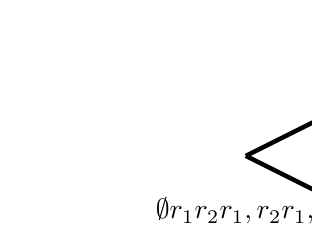
\begin{tikzpicture}[scale=0.8]
        \crd{0}{0}{$\emptyset$}
        \crd[left]{-2}{1}{$\s{r_1}$}
        \crd[right]{2}{1}{$\s{r_2}$}
        \crd[right]{0}{2}{$\s{r_1,r_2}$}
        \crd[right]{0}{3}{$\s{r_1,r_2,u}$}
        \draw [ultra thick] (0,0) -- (2,1);
        \draw [ultra thick] (0,0) -- (-2,1);
        \draw [ultra thick] (-2,1) -- (0,2);
        \draw [ultra thick] (2,1) -- (0,2);
        \draw [ultra thick] (0,2) -- (0,3);
    \end{tikzpicture}
    \caption{}
    \label{fig:es:configs}
\end{figure}

\begin{figure}
    \centering
    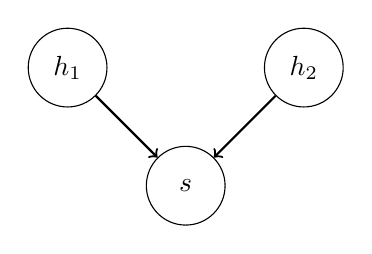
\begin{tikzpicture}[node distance={15mm},minimum size=10mm,
            main/.style = {draw, circle}]
        \node[main] (S)  {$s$};
        \node[main] (H1) [above of=S,left of=S] {$h_1$};
        \node[main] (H2) [above of=S,right of=S] {$h_2$};
        \draw[->,thick] (H1) -- (S);
        \draw[<-,thick] (S) -- (H2);
    \end{tikzpicture}
    \caption{}
    \label{fig:es:update}
\end{figure}

\section{مدل علّی}
پیدا کردن تعریفی برای علت واقعی
\lf{Actual Cause}
مبحثی است که مورد مطالعه و تحقیق بسیاری قرار گرفته است.
این مساله به طور خاص در متون فلسفه مورد توجه قرار گرفته است.
یکی از تعاریف علت واقعی که مورد توجه بسیاری قراری گرفته است، تعریفی مبتنی بر وابستگی خلاف واقع
\lf{Counterfactual}
است.
مطابق این تعریف، رویداد الف علت رویداد ب است اگر در شرایطی که رویداد الف اتفاق نیافته باشد، رویداد ب هم اتفاق نیافتند.
در اینجا اتفاق نیفتادن رویداد الف خلاف واقع است، چون در سناریوی واقعی
(سناریو ای که واقعا اتفاق افتاده و مشاهده شده است)
رویداد الف اتفاق افتاده است و در نظر گرفتن شرایطی که در آن رویداد الف اتفاق نیفتاده باشد بر خلاف واقعیت موجود است.
اما این مدل به تنهایی امکان پیدا کردن علت مناسب را در همه‌ی موارد ندارد.
به عنوان مثال سناریوی زیر را در نظر بگیرید که در آن سارا و بهرام هر کدام یک سنگ را برداشته و به سمت یک بطری شیشه‌ای پرتاب می‌کنند.
در این سناریو، سنگ سارا زودتر از سنگ بهرام به بطری برخورد کرده و در نتیجه آن را می‌شکند.
در این سناریو واضح است که پرتاب سنگ توسط سارا علت شکسته شدن بطری است.
فرض کنید بخواهیم از علیت مبتنی بر خلاف واقع برای پیدا کردن این علت استفاده کنیم.
بنابراین باید شرایطی را در نظر بگیریم که سارا سنگ خود را پرتاب نکند.
اما مشکل اینجاست که در این شرایط همچنان بطری شکسته می‌شود، چون اگر سارا سنگ خود را پرتاب نکند، بهرام همچنان سنگ خود را پرتاب می‌کند و در نتیجه این بار سنگ بهرام به بطری برخورد کرده و آن را می‌شکند.
بنابراین در این سناریو امکان تعریف پرتاب سنگ توسط سارا به عنوان علت شکسته شدن بطری با استفاده از استدلال مبتنی بر خلاف واقع وجود ندارد.
هالپرن
\lf{Halpern}
و پرل
\lf{Pearl}
برای حل کردن مشکلاتی از این دست، تعریف جدیدی از علت واقعی
\cite{hp}
ارائه کردند.
مدل ارائه شده توسط آن‌ها به دلیل اینکه مبنای ریاضی دارد امکان استفاده از آن را در آنالیز و تحلیل سیستم‌های محاسباتی فراهم می‌کند.
به همین دلیل این تعریف در مقالات زیادی در حوزه‌ی دانش کامپیوتر مورد استفاده قرار گرفته است.
برای تعریف علت واقعی ابتدا برخی مفاهیم اولیه مورد استفاده در این تعریف توضیح داده می‌شوند.
به صورت کلی فرض می‌شود که دنیای مورد تحلیل توسط تعدادی متغیر تصادفی مدل شده است.
اگر
$X$
یک متغیر تصادفی باشد، یک رویداد به شکل
$X=x$
تعریف می‌شود.
برخی از این متغیر‌ها بر روی یکدیگر تاثیر گذارند.
این وابستگی‌ها در قالب مجموعه‌ای از معادلات ساختاری
\lf{Structural Equations}
مدل می‌شوند.
هر یک از این معادلات در واقع یک مکانیزم یا قانون مشخص در این دنیا را مدل می‌کنند.
متغیرها به دو دسته درونی
\lf{Endogenous}
و برونی
\lf{Exogenous}
تقسیم می‌شوند.
متغیر‌های برونی متغیر‌هایی در نظر گرفته می‌شوند که مقدار آن‌ها توسط عواملی که درون مدل نیستند تعیین می‌شوند.
بنابراین در یک مدل علی فرض می‌شود که مقدار این متغیر‌ها از قبل مشخص است.
اما متغیر‌های درونی متغیرهایی هستند که مقدار آن‌ها بر اساس معادلات ساختاری تعیین می‌شود.
به صورت دقیق‌تر، امضای
\lf{Signature}
یک مدل یک سه‌تایی
$\mc{S} = (\mc{U},\mc{V},\mc{R})$
است که در آن
$\mc{U}$
مجموعه‌ی متغیر‌های بیرونی
$\mc{V}$
مجموعه‌ی متغیر‌های درونی و
$\mc{R}$
دامنه‌ی مقادیر ممکن برای هر یک از متغیر‌ها را مشخص می‌کند.
در این مدل فرض می‌شود که مجموعه‌ی متغیر‌های درونی محدود است.
مدل علّی بر روی یک امضای
$\mc{S}$
یک دوتایی
$\mc{M} = (\mc{S},\mc{F})$
است که در آن
$\mc{F}$
به هر متغیر داخلی
$X \in \mc{V}$
یک تابع
$F_X: \times_{Z\in ((\mc{U}\cup \mc{V})\setminus \s{X})}R(Z)
\rightarrow \mathcal{R}(X)$
اختصاص می‌دهد.
نشانه‌گذاری
$\times_{Z\in ((\mc{U}\cup \mc{V})\setminus \s{X})}$
ضرب خارجی
\lf{Cross-Product}
مجموعه‌های
$\mc{R}(Z)$
را به ازای تمام متغیر‌هایی مانند 
$Z$
در 
$(\mc(U)\cup \mc{V}) \setminus \s{X}$
مشخص می کند.
بنابراین اگر فرض کنیم
$(\mc{U}\cup \mc{V})\setminus \s{X} = \s{Z_1,...,Z_k}$
، آنگاه 
$\times_{Z\in ((\mc{U}\cup \mc{V})\setminus \s{X})}\mc{R}(Z)$
متشکل از چندتایی‌هایی به شکل
$(z_1,...,z_k)$
است که به ازای 
$i = 1,...,k$
هر 
$z_i$
یک مقدار ممکن برای متغیر 
$Z_i$
است.
هر تابع، معادله‌ی یک متغیر را به ازای مقادیر تمام متغیر‌های دیگر مشخص می‌کند.
به عنوان مثال اگر فرض کنیم
$F_X(Y,Z,U) = Y + U$
اگر داشته باشیم
$Y=3, U=2$
آنگاه مقدار
$X$
برابر ۵ خواهد شد.
این معادلات امکان تفسیر آن‌ها بر اساس شرایط خلاف واقع را می‌دهند.
به عنوان مثال در همین مدل اگر فرض کنیم که
$U=u$
می‌توانیم نتیجه بگیریم که اگر مقدار متغیر
$Y$
برابر ۴ باشد آنگاه مستقل از اینکه مقدار بقیه‌ی متغیر‌ها در دنیای واقعی چه مقداری دارند، مقدار متغیر
$X$
برابر
$u+4$
خواهد بود که به صورت
$(M,u) \vDash [Y \la 4](X = u + 4)$
نوشته می‌شود.
توابع ذکر شده فقط برای متغیر‌های درونی تعریف می‌شوند و همانطور که پیش‌تر اشاره شد، برای متغیرهای بیرونی تابعی تعریف نمی‌شود و فرض می‌شود که مقدار آن‌ها از قبل مشخص شده است
\cite{Halpern_2016}.

\begin{example}
      \label{ex:hp:fire}
      یک جنگل را در نظر بگیرید که می‌تواند توسط رعد و برق یا یک کبریت رها شده دچار آتش سوزی شود.
      برای مدل کردن این سناریو از سه متغیر بولی
      \lf{Boolean}
      استفاده می‌کنیم:
      \begin{itemize}
            \item متغیر
                  $F$
                  که اگر جنگل دچار آتش سوزی شود مقدار آن درست است و در غیر این صورت مقدار آن غلط است
            \item متغیر
                  $L$
                  که اگر رعد و برق اتفاق افتاده باشد مقدار آن درست است و در غیر این صورت غلط است
            \item متغیر
                  $M$
                  که اگر یک کبریت در جنگل رها شده باشد مقدار آن درست است و در غیر این صورت غلط است
      \end{itemize}
\end{example}
در این مثال فرض می کنیم که مقادیر متغیر‌های برونی به گونه‌ای است که تمام شرایط لازم برای آتش سوزی جنگل در صورتی که رعد و برق اتفاق بیافتد یا کبریتی در جنگل رها شود را دارد
(به عنوان مثال درختان جنگل به اندازه‌ی کافی خشک هستند و اکسیژن کافی در هوا وجود دارد).
در این مدل تابع متغیر
$F$
را به گونه‌ای تعریف می‌کنیم که داشته باشیم:
$F_F(\vec u, L , M) = L \vee M$.
همانطور که پیش‌تر بیان شد، این مدل علّی امکان بررسی معادلات بر اساس شرایط خلاف واقع را می‌دهد.
به صورت دقیق‌تر اگر
$M = (\mc{S},\mc{F})$
یک مدل علی،
$\vec X$
یک بردار از متغیرهای درونی و
$\vec{x}, \vec{u}$
برداری از مقادیر متغیر‌های
$\vec{X},\mc{U}$
باشند
مدل
$M_{\vec{X}\la \vec{x}}$
را با امضای
$S_{\vec X}=(\mc{U},\mc{V}-\vec X,\mc{R}|_{\mc{V} \setminus \vec{X}})$
یک زیرمدل
\lf{Sub-Model}
از
$M$
تعریف می‌کنیم که در آن
$\mc{R}|_{\mc{V}\setminus \vec X}$
محدود کردن 
$\mc{R}$
به متغیر‌های داخل 
$\mc{V} \setminus \vec X$
است.
به صورت شهودی این مدل حاصل مداخله‌
\lf{Intervention}
ای در مدل
$M$
است که در آن مقادیر
$\vec{x}$
را به متغیر‌های
$\vec{X}$
اختصاص داده‌ایم.
به صورت دقیق‌تر تعریف می‌کنیم
$M_{\vec{X}\la\vec{x}} = (\mc{S}_{\vec{X}},\mc{F}^{\vec{X}\la\vec{x}})$
که
$F_Y^{\vec{X}\la\vec{x}}$
از تابع
$F_Y$
که در آن مقادیر
$\vec{x}$
را به متغیرهای
$\vec{X}$
اختصاص داده‌ایم به دست می‌آید.
به عنوان مثال اگر
$M$
مدل مثال
\ref{ex:hp:fire}
باشد آنگاه در مدل
$M_{L\la \F}$
معادله‌ی متغیر
$F$
به
$F = M$
تبدیل می‌شود.
این معادله دیگر به متغیر
$L$
وابسته نیست بلکه با توجه به مقدار آن که در اینجا غلط است معادله‌ی جدیدی دارد.
علاوه براین توجه کنید که در مدل
$M_{L\la \F}$
دیگر معادله‌ای برای متغیر
$L$
وجود ندارد.
توجه کنید که در حالت کلی ممکن است یک بردار یکتا از مقادیر متغیر‌ها برای یک مدل وجود نداشته باشد که همزمان تمامی معادلات را حل کند.
در مدل علّی یک بردار از مقادیر متغیر‌های برونی
$\vec u$
یک هم‌بافت
\lf{Context}
نامیده می‌شود.
در مدل‌های بازگشتی به ازای یک هم‌بافت مشخص همیشه یک راه‌حل یکتا برای تمامی معادلات مدل وجود دارد.
در ادامه فرض می‌شود که مدل‌ها بازگشتی هستند. تعمیم مدل‌ علّی برای مدل‌های غیربازگشتی در
\cite{hp}
توضیح داده است.
برای یک مدل می‌توان یک شبکه‌ی علّی ترسیم کرد.
این شبکه یک گراف جهت‌دار است که به ازای هر متغیر یک گره در آن وجود دارد و یک یال بین دو گره وجود دارد اگر تابع متغیر دوم به متغیر اول وابسته باشد.
به عنوان مثال شکل زیر شبکه‌ی علّی مثال
\ref{ex:hp:fire}
را نشان می‌دهد:
\begin{center}
      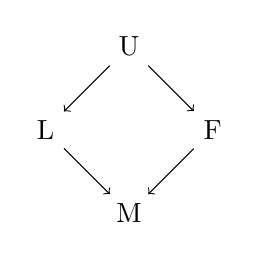
\begin{tikzpicture}[node distance={15mm}]
            \node (l) {L};
            \node (m) [below right of=l]  {M};
            \node (f) [above right of=m] {F};
            \node (u) [above right of=l] {U};
            \draw [->] (l) -- (m);
            \draw [->] (f) -- (m);
            \draw [->] (u) -- (l);
            \draw [->] (u) -- (f);
      \end{tikzpicture}
\end{center}
در ادامه برای سادگی رسم شبکه‌ی علی، متغیر‌های برونی را از آن‌ها حذف می‌کنیم.
\subsection{علت واقعی}
در ادامه‌ فرمول‌های لازم برای تعریف علت واقعی توصیف می‌شوند.
اگر
$\mc{S} = (\mc{U},\mc{V},\mc{R})$
یک امضا باشد فرمول
‍‍$X=x$
یک رویداد بدوی
\lf{Prime Event}
نامیده می‌شود که
‍$X \in \mc{V},x \in \mc{R}(X)$.
فرمول
$[Y_1 \la y_1,...,Y_k\la y_k]\varphi$
یک فرمول علّی پایه
\lf{Basic Causal Formula}
نامیده می‌شود که در آن:
\begin{itemize}
      \item $\varphi$
            یک ترکیب بولی از رویداد‌های بدوی است
      \item $Y_1,...,Y_k$
            متغیر‌های متمایز در
            $\mc{V}$
            هستند
      \item $y_i \in \mc{R}(Y_i)$
\end{itemize}
این فرمول به صورت خلاصه به شکل
$[\vec{Y}\la \vec{y}]\varphi$
نوشته می‌شود و اگر
$k=0$
باشد آنگاه به صورت
$\varphi$
نوشته می‌شود.
به صورت شهودی یک فرمول به شکل
$[\vec{Y}\la \vec{y}]\varphi$
بیان می‌کند که در شرایط خلاف واقع‌ ای که در آن مقادیر
$\vec{y}$
به متغیر‌های
$\vec{Y}$
اختصاص داده شده است فرمول
$\varphi$
برقرار است.
یک فرمول علّی به صورت یک ترکیب بولی از فرمول‌های علّی پایه تعریف می‌شود.
برقراری فرمول علی
$\psi$
در مدل
$M$
تحت هم‌بافت
$\vec u$
را به صورت
$(M,\vec u) \vDash \psi$
نشان می‌دهیم.
به عنوان مثال
$(M,\vec{u}) \vDash [\vec{Y}\la \vec{y}](X=x)$
برقرار است اگر مقدار متغیر
$X$
در راه حل معادلات مدل
$M_{\vec{Y}\la \vec{y}}$
تحت هم‌بافت
$\vec u$
برابر
$x$
باشد.

\begin{definition}
      \label{def:cause}
      فرمول
      $\vec X = \vec x$
      علت واقعی
      $\varphi$
      (
      که تاثیر
      \lf{Effect}
      نامیده می‌شود)
      در
      $(M,\vec{u})$
      است
      اگر شرایط زیر برای آن برقرار باشد:
      \begin{enumerate}
            \item $(M,\vec{u}) \vDash (\vec{X} = \vec{x}) \wedge \varphi$
            \item یک افراز مانند
                  $(\vec{Z},\vec{W})$
                  از مجموعه‌ی متغیر‌های
                  $\mc{V}$
                  با شرط
                  $\vec{X} \subseteq \vec{Z}$
                  و مقادیر
                  $(\vec{x},\vec{w}')$
                  برای متغیر‌های
                  $(\vec{X},\vec{W})$
                  وجود داشته باشد که داشته باشیم
                  $(M,\vec{u})\vDash \vec{Z} = \vec{z}^*$
                  و شرایط زیر را برآورده کند:
                  \begin{enumerate}
                        \item $(M,\vec u)\vDash[\vec{X}\la\vec{x}',\vec{W}\la\vec{w}']
                                    \neg \varphi$
                        \item $\forall \vec{W'} \subseteq \vec{W},\vec{Z'}\in \vec{Z}.
                                    (M,\vec{u})\vDash [\vec X\la\vec x,\vec{W}'\la \vec{w}',\vec{Z}'\la \vec{z}^*]\varphi$
                  \end{enumerate}
            \item $\vec X$
                  مینیمال باشد.
      \end{enumerate}
\end{definition}
در این تعریف شرط اول بیان می‌کند که علت و تاثیر هر دو در شرایط واقعی برقرار هستند.
شرط دوم به دنبال پیدا کردن شرایطی است که تحت آن تاثیر به صورت غیر واقع به علت وابسته باشد.
این شرایط متغیرهای
$\vec W$
و مقادیری مانند
$\vec{w}'$
برای آن‌ها هستند.
شرط ۲.آ بررسی می‌کند که تحت شرایطی که توسط
$\vec W \la \vec{w}'$
به وجود می‌آید اگر علت مقداری متفاوت از مقدار خود در هم‌بافت واقعی داشته باشد اثر در مدل دیده نمی‌شود.
شرط ۲.ب بررسی می‌کند که شرایط
استفاده شده در ۲.آ عامل
از بین رفتن اثر در ۲.آ نباشند.
برای این منظور در شرایطی که علت مقدار واقعی خود را دارد در تمامی حالت‌هایی که متغیر‌های شرایط می‌توانند داشته باشند بررسی می‌شود که اثر همچنان برقرار باشد.
شرط سوم در واقع بیان می‌کند که زیرمجموعه‌ای از علت وجود نداشته باشد که همزمان شرایط ۱ و ۲ را برقرار کند.
در تعریف بالا
$(\vec W, \vec w',\vec x')$
یک شاهد
\lf{Witness}
بر اینکه
$\vec X = \vec x$
علت
$\varphi$
است تعریف می‌شود.

\subsection{پیدا کردن علت واقعی در مسائل}

در ادامه مثال سارا و بهرام که در ابتدای این بخش ذکر شده بود را بررسی می‌کنیم.

برای مدل کردن این مساله متغیر‌های زیر را در نظر می‌گیریم:
\begin{itemize}
      \item $BT$:
            پرتاب سنگ توسط بهرام
      \item $BH$
            برخورد سنگ بهرام به بطری
      \item $ST$:
            پرتاب سنگ توسط سارا
      \item $SH$:
            برخورد سنگ سارا به بطری
      \item $BS$:
            شکسته شدن بطری
\end{itemize}

\begin{figure}
      \centering
      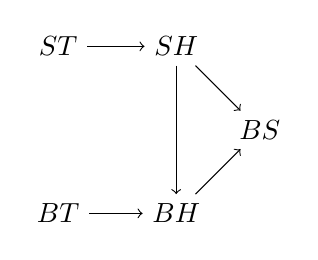
\begin{tikzpicture}[node distance={15mm}]
            \node (bs)  {$BS$};
            \node (sh) [above left of=bs] {$SH$};
            \node (bh) [below left of=bs] {$BH$};
            \node (st) [left of=sh]{$ST$};
            \node (bt) [left of=bh] {$BT$};
            \draw [->] (st) -- (sh);
            \draw [->] (sh) -- (bh);
            \draw [->] (bt) -- (bh);
            \draw [->] (sh) -- (bs);
            \draw [->] (bh) -- (bs);
      \end{tikzpicture}
      \caption{}
      \label{fig:hp:sb}
\end{figure}
ابتدا فرض می‌کنیم که متغیر‌های
$BT,ST$
تنها به متغیر‌های برونی وابسته‌اند.
بطری در صورتی شکسته می‌شود که هر یک از سنگ‌های سارا یا بهرام با آن برخورد کنند.
بنابراین برای شکسته شدن بطری معادله‌ی
$BS = BH \vee SH$
را در نظر می‌گیریم.
نکته‌ی اصلی در این مساله این است که سنگ سارا زودتر از سنگ بهرام به شیشه برخورد می‌کند، به همین دلیل لازم است تا این موضوع در مدل لحاظ شود.
یک راه برای مدل کردن این مساله این است که معادله‌ی برخورد سنگ بهرام به شیشه را به گونه‌ای تعریف کنیم که تنها در صورتی که سنگ سارا به بطری برخورد نکرده باشد آنگاه سنگ بهرام به بطری برخورد کند.
بنابراین می‌توانیم معادله‌ی
$BH = BT \wedge \neg SH$
را تعریف کنیم.
علاوه بر این معادله‌ی برخورد سنگ سارا را بدون وابستگی به برخورد سنگ بهرام تعریف می‌کنیم:
$SH = ST$.
با توجه به این تعاریف برای معادلات می‌توانیم گراف علّی شکل
\ref{fig:hp:sb}
را برای این مدل رسم کنیم
در این مدل می‌توانیم
$ST = \T$
را به عنوان علت
$BS = \T$
تعریف کنیم.
برای برقراری شرط ۲ در تعریف علت واقعی شرایط
$\vec W = \s{BT}$
و
$w' = \F$
را در نظر می‌گیریم.
در این شرایط چون مقدار
$BH$
برابر
$\F$
می‌شود، مقدار
$BS$
تنها وابسته به مقدار
$SH$
و در نتیجه
$ST$
می‌شود.
همچنین در این مدل
$BT = \T$
علت شکسته شدن شیشه نیست.
مثلا فرض کنید که شرایط
$\vec W = \s{ST},w' = \F$
را در نظر بگیریم.
در این شرایط اگر مقدار
$BT$
را به
$\F$
تغیر دهیم مقدار
$BS$
هم غلط می‌شود.
بنابراین شرط ۲.آ برقرار است.
اما به ازای
$\vec Z' = \s{BH}$
شرط ۲.ب برقرار نمی‌شود.
در این حالت داریم:
$(M,\vec{u})\vDash[BT \la \T,ST \la \F,BH \la F]BS = \F$
توجه کنید با وجود اینکه مقدار درست به
$BT$
اختصاص یافته اما چون مقدار
$BH$
به مقدار آن در هم‌بافت واقعی برگردانده می‌شود در نتیجه مقدار
$BS$
همچنان غلط می‌ماند.

مثال بالا نشان می‌دهد که این تعریف از علت واقعی برخی از مشکلات موجود در تعاریف ساده مبتنی بر خلاف واقع را برطرف می‌کند و می‌تواند توضیح مناسبی در برخی از این مثال‌ها پیدا کند.
نکته‌ای که باید به آن توجه شود این است که هنوز روش یا معیاری برای این که چه تعریفی از علت واقعی تعریف مناسب است وجود ندارد.
تنها روش ممکن مقایسه تعاریف مختلف استفاده از آن‌ها در مساله‌ها و سناریوهای مختلف و بررسی تطابق علت به دست آمده با استفاده از این تعریف‌ها با شهود موجود از مساله است.

\subsection{مدل تعمیم‌یافته}
مدل علّی تعمیم یافته
\lf{Extended Causal Model}
یک سه‌تایی
$(\mc{S},\mc{F},\mc{E})$
است که
$(\mc{S},\mc{F})$
یک مدل علّی است و
$\mc{E}$
یک مجموعه از مقداردهی‌های مجاز
\lf{Allowable Settings}
برای متغیر‌های درونی است.
به صورت دقیق‌تر اگر متغیر‌های درونی
$X_1,...,X_n$
باشند آن‌گاه
$(x_1,...,x_n) \in \mc{E}$
اگر
$X_1=x_1,...,X_n=x_n$
یک مقداردهی مجاز است.
یک مقداردهی دلخواه به یک زیرمجموعه از متغیر‌های درونی مجاز است اگر امکان تعمیم به یک مقداردهی مجاز در
$\mc{E}$
را داشته باشد.
هدف از این تعریف جلوگیری از در نظر گرفتن علت‌هایی است که شرایط رخ دادن آن‌ها غیر محتمل است.
با توجه به تعریف مقداردهی مجاز، علت واقعی در یک مدل تعمیم یافته به گونه‌ای تعریف می‌شود که در شرط ۲ فقط امکان مقداردهی‌های مجاز وجود داشته باشد.
در
\cite{hp}
تعریف دقیق علت واقعی در مدل تعمیم یافته بیان نشده است.
در بخش بعدی تعریفی از علت واقعی در مدل تعمیم یافته ارائه می‌شود.

\subsection{علت واقعی بدون شرط}
فرض کنید که
$\vec X = \vec x$
یک علت واقعی برای
$\varphi$
در
$(M,\vec u)$
با استفاده از شاهد
$(\e,\e,\vec x')$
باشد.
با توجه به اینکه در اینجا
$\vec W$
یک بردار خالی است پس عملا شرط ۲.ب به بررسی شرط زیر تبدیل می‌شود:
\begin{align*}
      \forall \vec{Z'}\in \vec{Z}.
      (M,\vec{u})\vDash [\vec X\la\vec x,\vec{Z}'\la \vec{z}^*]\varphi
\end{align*}
با دقت در شرط بالا می‌توان دریافت که مقدار متغیر‌ها در فرمول‌های
$[\vec X\la\vec x,\vec{Z}'\la \vec{z}^*]\varphi $
با مقدار متغیر‌ها در هم‌بافت اولیه تفاوتی ندارد زیرا مقدار آن‌ها به مقداری که در هم‌بافت اولیه داشته‌اند برگردانده می‌شود.
بنابراین در شرط بالا می‌توان نتیجه گرفت:
\begin{align*}
      (M,\vec{u})\vDash [\vec X\la\vec x,\vec{Z}'\la \vec{z}^*]\varphi 
      \iff (M,\vec{u}) \vDash \varphi
\end{align*}
بنابراین شرط ۲.ب معادل با شرط ۱ می‌شود.
با توجه به این موضوع می‌توان گزاره زیر را نتیجه گرفت:
\begin{proposition}
      \label{prop:but-for}
     اگر 
     $\vec X = \vec x$
     در 
     $(M,\vec u)$
     با شاهدی به شکل
     $(\e,\e,\vec x')$
     شرط‌های ۱، ۲.آ و ۳ در تعریف 
     \ref{def:cause}
     را برای 
     $\varphi$
     برآورده کند آنگاه 
     $\vec X = \vec x$
     یک علت واقعی برای 
     $\varphi$
     در 
     $(M,\vec u)$
     است.
\end{proposition}

